Рассмотрим движение в потенциальном поле
\begin{equation*}
    U(x) = - \frac{\hbar^2 \kappa_0}{m} \sum_{n=-\infty}^{\infty} \delta(x-n a).
\end{equation*}
Запишем стационарное уравнение Шрёдингера
\begin{equation*}
    \hat{H} = - \tfrac{\hbar^2}{2m} \partial_x^2 + U(x), 
    \hspace{10 mm} 
    \hat{H} \psi(x) = E \psi(x).
\end{equation*}
Подставляя, находим
\begin{equation*}
    \psi''(x) - \tfrac{2m}{\hbar^2} \left(U(x) - E\right) \psi(x) = 0,
    \hspace{0.5cm} \Rightarrow \hspace{0.5cm}
    \psi(x) = \left\{\begin{aligned}
        &\alpha_1 e^{i k x} + \beta_1 e^{- i k x}, &x \in [0, a]; \\
        &\alpha_2 e^{i k (x-a)} + \beta_2 e^{-ik (x-a)}, &x \in [a, 2a];
    \end{aligned}\right.
\end{equation*}
где рассмотрели решение на двух областях: $[0, a]$ и $[a, 2a]$, и ввели $k^2 = \frac{2m}{\hbar^2} E$. 

Запишем условие на непрерывность $\psi(x)$ и скачок первой производной
\begin{equation*}
    \left.\begin{aligned}
        \psi(a+\varepsilon) &= \psi(a-\varepsilon), \\
        \psi'(a+\varepsilon) - \psi'(a-\varepsilon) &= - 2 \kappa_0 \psi(a),
    \end{aligned}\right\}
    \hspace{0.5cm} \Rightarrow \hspace{0.5cm}
    \begin{pmatrix}
        \alpha_2 \\ \beta_2
    \end{pmatrix} = 
    A \begin{pmatrix}
        \alpha_1 \\ \beta_1
    \end{pmatrix},
    \hspace{5 mm} 
    A = \begin{pmatrix}
        \bp
        e^{ika}\left(1-\frac{\kappa_0}{ik}\right) & -e^{-ika} \frac{\kappa_0}{ik}  \\
        \bp
        e^{ika} \frac{\kappa_0}{ik} & e^{-ika} \left(1 + \frac{\kappa_0}{i k}\right)  \\
    \end{pmatrix}
\end{equation*}
Здесь, для удобства, ввели связь коэффициентов через матрицу $A$.


В силу периодичности потенциала, $[\hat{H},\, \hat{T}_a] = 0$, и решение может быть найдено в виде функций Блоха\footnote{
    Действительно, $\psi(x) = e^{K a} F(x)$, где $F(x+a) = F(x)$, тогда 
    $\psi(x+a) = e^{i K a} \psi(x)$.
} 
\begin{equation*}
    U(x+a) = U(x),
    \hspace{0.5cm} \Rightarrow \hspace{0.5cm}
    \psi(x+a) = e^{i K a} \psi(x).
\end{equation*}
Тогда, подставляя предполагаемое решение, находим
\begin{equation*}
    \begin{pmatrix}
        \alpha_2 \\ \beta_2
    \end{pmatrix} = e^{i K a} \begin{pmatrix}
        \alpha_1 \\ \beta_1
    \end{pmatrix}.
\end{equation*}
Получается, матрица $A$ должна быть скалярна, чего можем добиться дополнительными условиеями на $\alpha$ и $\beta$:
\begin{equation*}
    \lambda^2 - (\tr A) \lambda + \det (A) = 0,
    \hspace{5 mm} 
    \tr A = e^{i k a} \left(1 - \tfrac{\kappa_0}{ik}\right) + e^{-ika} \left(
        1 + \tfrac{\kappa_0}{ik}
    \right) \overset{\mathrm{def}}{=} 2 \rho,
    \hspace{5 mm} 
    \det A = 1.
\end{equation*}
Подставляя условие из $[\hat{H},\, \hat{T}_a] = 0$, находим 
\begin{equation*}
    \lambda_{1, 2} = e^{\pm i K a} = \rho \pm i \sqrt{1 - \rho^2},
\end{equation*}
что, вроде, носит гордое имя дисперсионного соотношения. Подставляя\footnote{
    Имеет смысл выразить $\rho = \cos(ak) - \frac{\kappa_0}{k} \sin(ak)$.
}  $\rho$ находим выражение для $K$:
\begin{equation*}
    \cos (Ka) = \cos (ka) - \tfrac{\kappa_0}{k} \sin (ka).
\end{equation*}
Так как $K a \in \mathbb{R}$, то дисперсионное соотношение становится условием на допустимые значения энергии и, из уравнения и достаточно убедительного рисунка, можем сделать вывод о разрешенных зонах. Действительно, для того, чтобы зона была разрешенной необходимо, чтобы
\begin{equation}
    |\cos (k[E] a) - \tfrac{\kappa_0}{k[E]} \sin (k[E]a)| < 1,
\end{equation}
на что чуть подробнее посмотрим в предельных случаях.

Построим $|\cos (k[E] a) - \tfrac{\kappa_0}{k[E]} \sin (k[E]a)|$ для $\kappa_0 a \ll 1$ (слабая связь) 
и $\kappa_0 a \gg 1$ (сильная связь). Видно, что слабой связи соответствует почти непрерывный спектр $\cos (Ka) \approx \cos (k a)$ и $K \approx k + \frac{2\pi n}{a}$, а сильная связб приводит к почти дискретному спектру с $ka \approx \pi n$. 
\begin{figure}[ht]
    \centering
    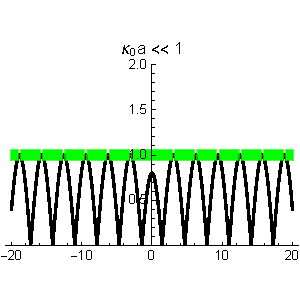
\includegraphics[width=0.3\textwidth]{figures/T7_1.pdf}
    \hspace{5 mm} 
    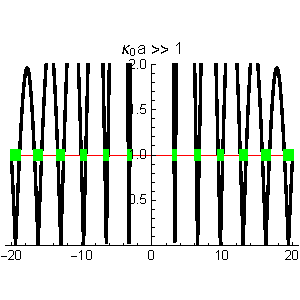
\includegraphics[width=0.3\textwidth]{figures/T7_2.pdf}
    \caption{Слабая и сильная связь в задаче Т7}
    %\label{fig:}
\end{figure}

% При малых значениях квазиимульса $K$ можем явно найти
% \begin{equation*}
%     K^2 = \frac{2 \kappa _0 \sin (k)}{a^2 k}-\frac{2 \cos (k)}{a^2}+\frac{2}{a^2},
% \end{equation*}
% что соответствует эффективной массе частицы.
По определению, эффективной массой частицы называется
\begin{equation*}
    m^* \overset{\mathrm{def}}{=} \hbar^2 \left(\frac{d^2 E}{d K^2} \right)^{-1},
\end{equation*}
где $\hbar K$ -- квазиимпульс. 

Считая $k$ малым, находим
\begin{equation*}
    \frac{1}{6} k^2 \left(a^3 \kappa _0-3 a^2\right)-a \kappa _0+1=\cos (a K),
    \hspace{0.5cm} \Rightarrow \hspace{0.5cm}
    E(K) = \frac{\hbar^2}{2m} k^2 = \frac{\hbar^2}{2m} \frac{6}{a^2} \frac{1 - \cos(K a) - a \kappa_0}{3 - \kappa_0 a}.
\end{equation*}
Тогда эффективная масса система равна
\begin{equation*}
    E''_{KK} = \frac{3 \hbar ^2 \cos (a K)}{m \left(3-a \kappa _0\right)}
    , \hspace{0.5cm} \Rightarrow \hspace{0.5cm}
    m^*= m \frac{1 - a \kappa_0/3}{\cos(a K)},
\end{equation*}
которое $a \kappa_0 \ll 1$ и $a K \ll 1$ переходит в классический случай! 
